%
% File naacl2019.tex
%
%% Based on the style files for ACL 2018 and NAACL 2018, which were
%% Based on the style files for ACL-2015, with some improvements
%%  taken from the NAACL-2016 style
%% Based on the style files for ACL-2014, which were, in turn,
%% based on ACL-2013, ACL-2012, ACL-2011, ACL-2010, ACL-IJCNLP-2009,
%% EACL-2009, IJCNLP-2008...
%% Based on the style files for EACL 2006 by 
%%e.agirre@ehu.es or Sergi.Balari@uab.es
%% and that of ACL 08 by Joakim Nivre and Noah Smith

\documentclass[11pt,a4paper]{article}
\usepackage[hyperref]{emnlp-ijcnlp-2019}
\usepackage{times}
\usepackage{latexsym}

\usepackage{url}

%\aclfinalcopy % Uncomment this line for the final submission

%\setlength\titlebox{5cm}
% You can expand the titlebox if you need extra space
% to show all the authors. Please do not make the titlebox
% smaller than 5cm (the original size); we will check this
% in the camera-ready version and ask you to change it back.

\newcommand\BibTeX{B{\sc ib}\TeX}
\newcommand\confname{EMNLP-IJCNLP 2019}
\newcommand\conforg{SIGDAT}
\usepackage{amsmath,amsthm,amsfonts,amssymb,amscd}
\usepackage{graphicx}
\usepackage{multirow}
\usepackage{url}
\usepackage{float} 
\usepackage{tabularx}
\usepackage{xcolor}
\newtheorem{lemma}{Lemma}[section]
\newtheorem{theorem}{Theorem}[section]
\newtheorem{proposition}{Proposition}[section]
\newtheorem{definition}{Definition}[section]
\DeclareMathOperator*{\argmax}{argmax}
\DeclareMathOperator*{\argmin}{argmin}
\usepackage{algorithm}
\usepackage{algorithmic}
\usepackage[draft]{todo}
\floatname{algorithm}{Procedure}
\renewcommand{\algorithmicrequire}{\textbf{Input:}}
\renewcommand{\algorithmicensure}{\textbf{Output:}}
%\aclfinalcopy % Uncomment this line for the final submission
%\def\aclpaperid{***} %  Enter the acl Paper ID here

\newcommand{\fyTodo}[1]{\Todo[FY:]{\textcolor{orange}{#1}}}
\newcommand{\fyTodostar}[1]{\Todo*[FY:]{\textcolor{orange}{#1}}}
\newcommand{\fyDone}[1]{\done[FY]\Todo[FY:]{\textcolor{orange}{#1}}}
\newcommand{\fyDonestar}[1]{\done[FY]\Todo[FY:]{\textcolor{orange}{#1}}}

%\setlength\titlebox{5cm}
% You can expand the titlebox if you need extra space
% to show all the authors. Please do not make the titlebox
% smaller than 5cm (the original size); we will check this
% in the camera-ready version and ask you to change it back.

\title{Sparse Word Embeddings for Multi-domain Machine Translation}

\author{First Author \\% Minh Quang Pham\\
  Affiliation / Address line 1 \\
  Affiliation / Address line 2 \\
  Affiliation / Address line 3 \\
  {\tt email@domain} \\\And
  Second Author \\
  Affiliation / Address line 1 \\
  Affiliation / Address line 2 \\
  Affiliation / Address line 3 \\
  {\tt email@domain} \\}

\date{}

\begin{document}
\maketitle

\fyDone{s/naacl/EMNLP/g}
\fyDone{Too long, selfcontained, noref, rewrite}
\begin{abstract}
  Supervised machine translation is well suited to the situation where the training and testing data are from the same domain. When this is not the case, \emph{domain adaptation} techniques are needed to ensure that the knowledge of the source, out-of-domain data, generalizes properly to the target, in domain, texts. We study a related setting, multi-domain adaptation, where the number of domains is potentially large, and where adapting separately to each woud waste training resources. Our proposal transposes to neural machine translation the feature expansion technique of (Daum\'e, 2007), and isolate domain-agnostic from domain-specific lexical representations, while sharing the rest of the architecture across domains. Our experiments use two standard architecture and two language pairs: they show that our approach, while remaining simple and computationally unexpensive, outperforms several strong baselines, and delivers a multi-domain system that can sucessfully process heterogeneous input sentences.

  THIS IS THE OLD ABSTRACT 
  Fine-tuning a generic neural machine translation model to a certain domain usually degrade its performance on the other domains, thus it's very difficult to build a unique model which is best for all. Indeed, Catastrophic Forgetting, well-known problem in Machine Learning, states that standard backprogation neural network suffers a lot while there is a shift in training data distribution. However, Finetuning is very costly and unefficient in the industry therefore one best model is always desired. In this paper, we introduce an application of an old technique \cite{Daume07frustratingly} in Multi-Domain Neural Machine Translation. By defining general information encoding region and domain-specific encoding region in word embedding vector, we are able to seperate domain-related information flows in forward and backward propagation during training thus to
mitigate the catastrophic interference happens during the training over different domains. Empirically, we achieved a unique model that has comparable score to finetuned models for every domains. Furthermore, our method is simple and could be applied to any architecture.
\end{abstract}

\section{Introduction \label{sec:introduction}}
% The problem
Owing to the development of flexible and powerful architectures based on neural networks \cite{Cho14properties,bahdanau2014neural,Ghering17convolutional,Vaswani17attention}, Machine Translation (MT) has made significant progress over the past years, and constitute the standard for most production engines to-date. One issue which repeatedly pops up with MT, be it neural or statistical, is the need to perform training with large parallel corpora, typically consisting of millions of parallel sentences deemed to be as close as possible to the application domain. A lot of the recent research effort has thus focused on developping MT systems in low data conditions, for instance building multilingual MTs, thereby enabling zero-shot translation \cite{Firat16multiway,Johnson17google} or even building systems without any parallel data \cite{Artetxe18unsupervised,Lample18unsupervised}.
Another important scenario for industrial MT systems is to adapt an neural system trained using a parallel data in one  domain to the peculiarity of other domains. Domain Adaption (DA) in MT is an old issue \cite{Foster07mixture,Axelrod11domain}, which comes in various guises, and for which a number of solutions have been studied (see the recent survey of \cite{Chu18asurvey} for neural MT). The typical setting is \emph{supervised adaptation}, where a (small) amount of data of the target domain of interest is used to fine-tuned the parameters of a system trained on a large amount of texts in a source domain. We study here a different scenario, multi-domain adaptation \cite{Farajian17multidomain}, where we would like to use heterogenous data sources to train a unique system that would work well for all domains. This allows us to be both data efficient (all data is used to train all domains) and compuationally efficient (we only need to train one domain). In our setting, we assume that the domain of test documents is known in advance.

Multi-domain adaptation is conceptually close to multilingual MT, or more generally to multi-task learning \cite{Caruana97multitask}, and can be approached in a number of ways. We adapt here the of \cite{Daume07frustratingly} to neural MT, in an attempt to confine the differences between domains at the lexical level, while the rest of the parameters is shared between domains. Our main hypothesis is that most of the differences between domains take place at the lexical level, due to massive cross-domain polysemy. By contrast, the deeper layers, which arguably model more abstract linguistic phenomena, should be made shareable across domains.
To this end, we make sure to design word embeddings in such that they will contain a generic as well as a domain-specific region. We perform experiments with three domains, two architectures and two language pairs and find that our technique can effectively build multi-domain NMT, outperforming several baselines. Our contribution is thus twofold:
\begin{itemize}
\item methods to adapt the ideas of \cite{Daume07frustratingly} for two NMT architectures;
\item experimental results that demonstrate the effectiveness of this technique;
\end{itemize}
\fyTodo{can we train in random order ? can we get away with catastrophic forgetting ?}
\fyTodo{how to analyze the embeddings ? how can we test or claim ?}

\section{Sparse embeddings \label{sec:sparse_embeddings}}
\fyDone{Use meaningful titles throughout}

\subsection{Problem statement}
\fyTodo{Use math for notation, label equations and such}
\begin{definition}{Domain}
\label{def:domain}
A domain is probabilistic distribution of translation $(x,y)$ in a given corpora. Given corpora $C$, we denote $D(C)$ the domain of $C$.
\end{definition}
\fyTodo{We need more: the source, the target, etc}
In machine translation, the loss function for training is:
\begin{equation}\label{eq:1}
\begin{split}
E_{(x,y) \sim p_{rel}}[-log(p_{\theta}(y|x))] &= \\
= E_{x \sim p_{rel}(x)}[KL(p_{rel}(y|x) & \mid p_{\theta}(y|x))] + \\
+ E_{x \sim p_{rel}} &[H(p_{rel}(y|x))]
\end{split}
\end{equation}.

Where $p_{\theta}(y|x) = p(y|x,\theta)$ \\
In this equation, the domain is $p_{rel}(x,y)$. In minimizing given objective \ref{eq:1}, one aims to approximate the objective domain $p_{rel}$. In inference, provided the model was trained on certain training data, the more likely test set is generated from domain of training data, the better performance.\\
In general, a generic model is trained first with a mix of several corpora which belongs to different topics (e.g medical, banking, adminstration) whose the domain $p_{rel}$ is considered as a general domain, noted $p_{gen}$. Being trained with a general mixed corpora, the generic model is not usually good enough for translating by topic. In order to improve topical translation quality, specializing generic model is required. One usually finetunes the generic model by continue the training from initial value $\theta^*$, which was optimized on general domain, using corpora of interested topic. However, there is always a dramatical shift from generic domain $p_{gen}$ to specialization domain $p_{spec}$. Indeed, the translation $(x,y)$ could be very different in different topic. For instance, in financial document, to translate "security" into "titre financier" is more likely than to translate it into "securit\'e" but in IT document. Therefore, the shift from general domain containing these two corpora to one of them is not negligible. This shift usually leads to catastrophic forgetting in neural network using backpropagation \cite{McCloskey1989Catastrophic}. In effect, the finetuned model usually shows lower performance in translating sentences, which are less related to the finetuning topic, than generic model. 
In order to conduct the model translating topic by topic, we might refer to conditional probability conditioned by topic $p(y|x,d)$. Given a set of training corpora, we assume that there are a limited d engendering topic, i.e, there are d corpora $C_i$ $i \in [1,..,d]$ representing d topical domains $D(C_i)$ respectively. We are then interested in approximating $p(y,x|i)$ for $i \in [1,..,d]$ and use $p(y|x,i)$ for the inference in topic $i$. From now, we formalize the multi-domain problem for machine translation in following equation
\begin{equation} \label{eq:2}
\begin{split}
\theta^* = \argmin_{\theta} \displaystyle{\mathop{\sum}_{i \in [1..d]}} E_{(x,y) \sim D(C_{i})}[-log(p_{\theta}(y|x,i))]
\end{split}
\end{equation}
It is obvious that
\begin{equation} \label{eq:3}
\begin{split}
\argmin_{\theta} \displaystyle{\mathop{\sum}_{i \in [1..d]}} E_{(x,y) \sim D(C_{i})} &[-log(p_{\theta}(y|x,i))] \\
\geq \displaystyle{\mathop{\sum}_{i \in [1..d]}} \argmin_{\theta} E_{(x,y) \sim D(C_{i})} &[-log(p_{\theta}(y|x,i))]
\end{split}
\end{equation}
A trivial solution for the equation \ref{eq:2} is $\theta^* = (\theta^*_{0},...,\theta^*_{d})$ and $p_{(\theta_{0},...,\theta_d)}(y|x,i)$ is independent of $\theta_{j}$ $\forall j \neq i$, i.e, $\exists f:\Omega_i \times C(D_i) \rightarrow [0,1]: f_{\theta_i}(y,x) = p_{(\theta_{0},...,\theta_d)}(y|x,i)$ where $\Omega_i$ is set of all possible values of $\theta_i$. \\
The trivial solution is not rather than ensemble of $d$ models specialized for one domain. However, we could reduce the seperation by using shared paramaters denoted $\theta_s$ then reformulate the model as following: \\
$\theta^* = (\theta^*_{0},...,\theta^*_{d}, \theta_s^*)$ and $p_{(\theta_{0},...,\theta_d, \theta_s)}(y|x,i)$ is independent of $\theta_{j}$ $\forall j \neq i$, i.e, $\exists f:\Omega_i \times \Omega_s \times C(D_i) \rightarrow [0,1]: f_{\theta_i, \theta_s}(y,x) = p_{(\theta_{0},...,\theta_d, \theta_s)}(y|x,i)$ \\ $p_{(\theta_{0},...,\theta_d, \theta_s)}(y|x)$ is independent of $\theta_{j}$ $\forall j$ i.e, $\exists \bar{f}:\Omega_s \times C \rightarrow [0,1]: \bar{f}_{\theta_s}(y,x) = p_{(\theta_{0},...,\theta_d, \theta_s)}(y|x)$
where $\Omega_i$ is set of all possible values of $\theta_i$ and $\Omega_s$ is set of all possible values of $\theta_s$. The optimization problem will become
\begin{equation}
\displaystyle{\mathop{\sum}_{i \in [1..d]}} \argmin_{\theta_{0},...,\theta_{d}, \theta_s} E_{(x,y) \sim D(C_{i})} [-log(p_{\theta_s,\theta_i}(y|x,i))]
\end{equation}
However, the couple $\theta_s^*$ and $\theta_i^*$ are hardly optimal $\forall i \in [1..d]$.\\
Despite the fact that $\theta^* = (\theta^*_{0},...,\theta^*_{d}, \theta_s^*)$ is hardly achieved by backpropagation, we could attempt to optimize $\theta_s$:
\begin{equation}
\theta^*_{s} = \displaystyle{\mathop{\argmin}_{\theta_s}}E_{(x,y) \sim D(\displaystyle{\mathop{\cup}_{i \in [1,..,d]}}C_{i})}[-log(p_{\theta_s}(y|x))]
\end{equation} 

then optimize each $\theta_i$ (as additional factor used for fine-tuning the model to the domain $D(C_{i})$) the perplexity with respect to true distribution of domain
\begin{equation}
\theta^*_{i} = \displaystyle{\mathop{\argmin}_{\theta_i}}E_{(x,y) \sim D(C_{i})}[-log(p_{\theta_i,\theta^*_s}(y|x,i))]
\end{equation} 
Our first approach to multi-domain machine translation is to build such trivial solution by assigning different regions of word embedding vector to set of domain paramters $\theta_i$ and set of shared parameters $\theta_s$ while keep sharing other parameters between domains.
\subsection{Sparse word embedding}
\label{sec:sparse}
This section explains a new design for word embedding used in multi-domain model. As mentioned above, we separate parameter set into $D+1$ parameter sets correspond to D domains and one shared paramater set. Our first attempt is to split standard vector word embedding into $D+1$ regions named $\theta_i$ for $i \in [1,..,D]$ and $\theta_s$.
\begin{figure}[h]
\center
    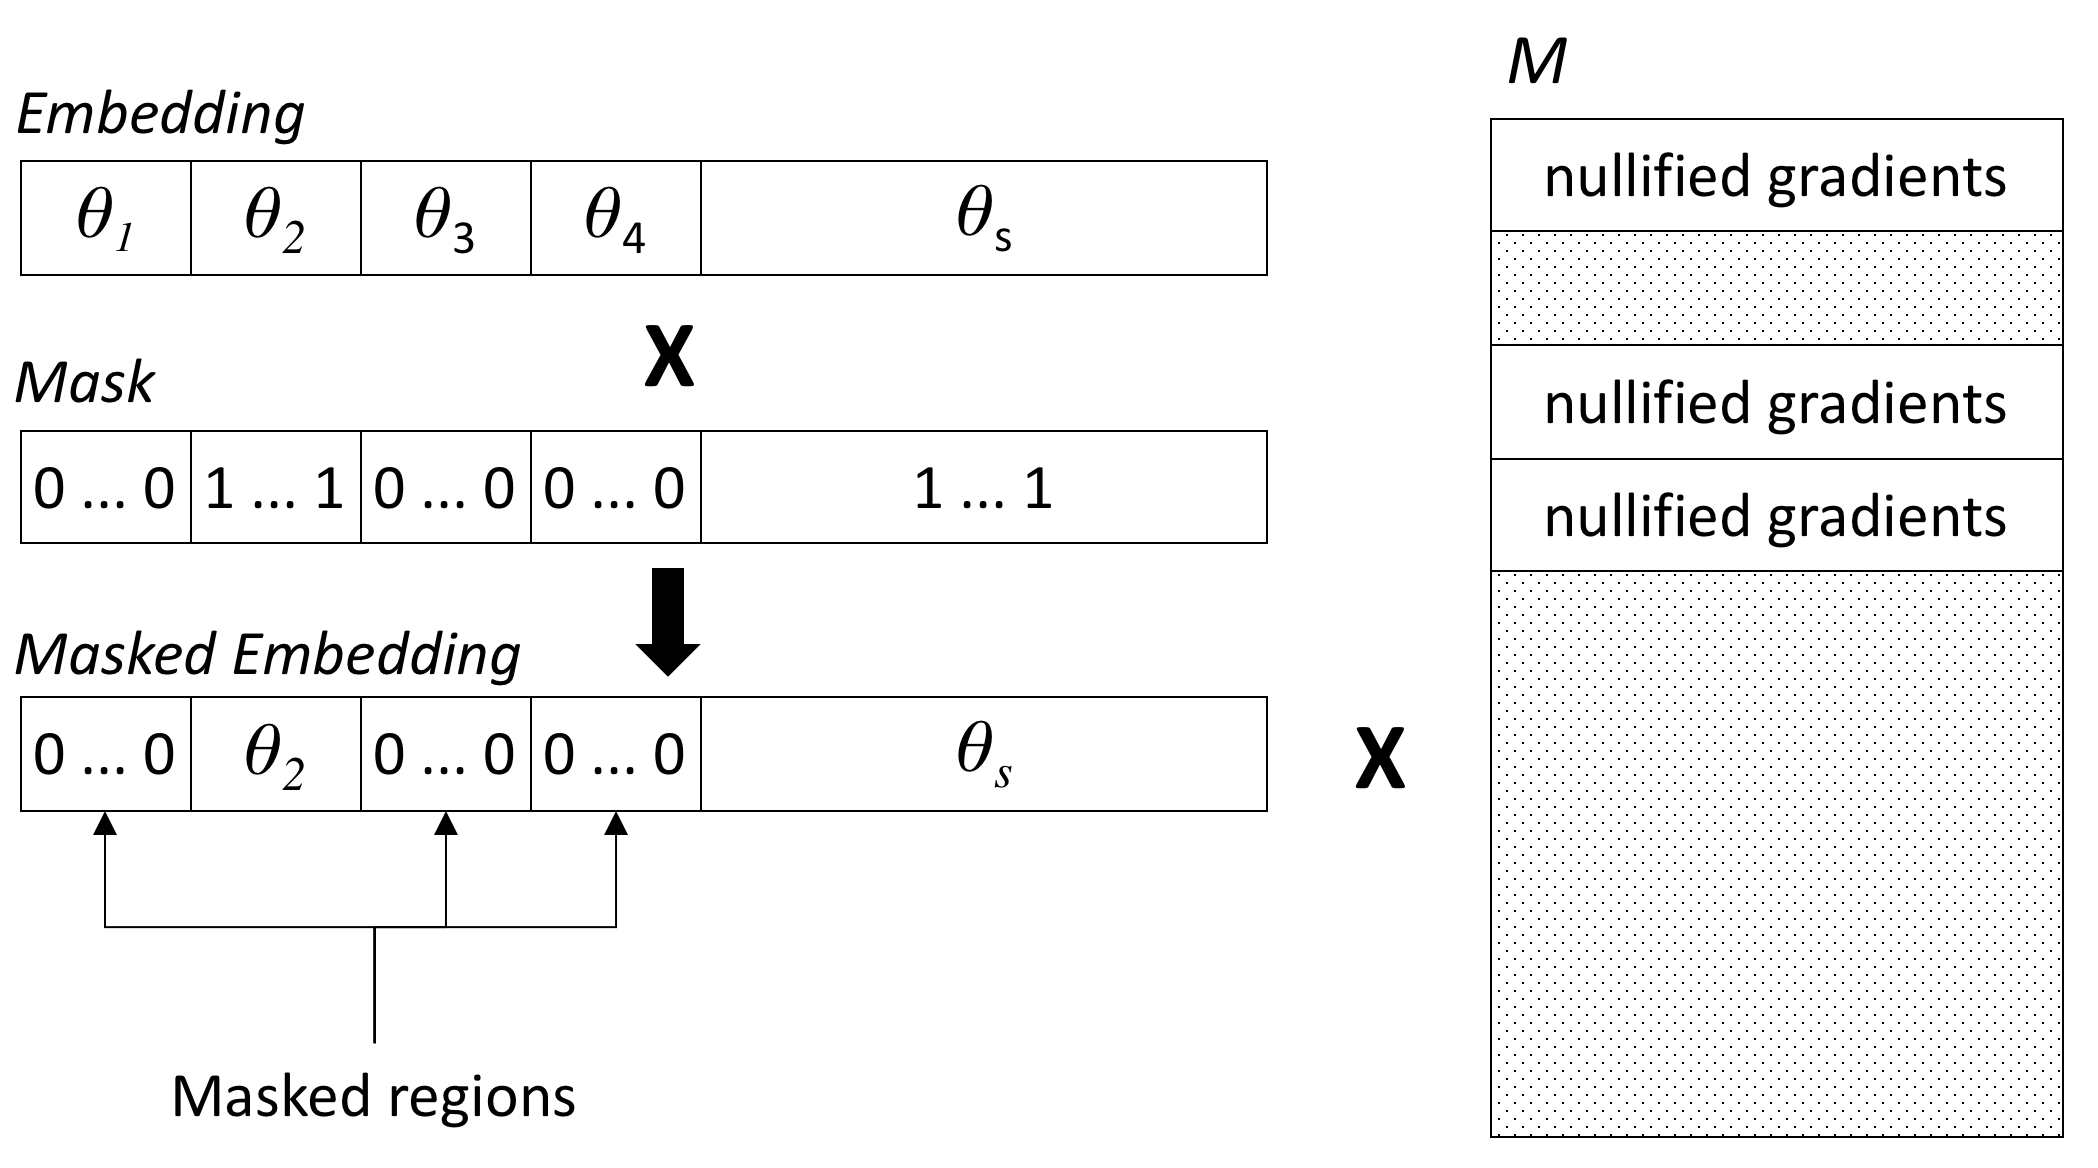
\includegraphics[width=\linewidth]{embeddings}
    \caption{Sparse word embeddings. The red region contains units that are activated only when an input from the corresponding domain is presented; the other (green) regions are deactivated; the blue (generic) region is always activated.} 
    \label{fig:network}
  \end{figure}
\fyTodo{Explain vanishing ?}
Figure~\ref{fig:network} presents our proposed design. During backprogation, the \fyTodo{fix notation}{projection matrix $M$} receives gradient 0 at regions corresponding to deactivated regions in the word embedding. Those regions are also masked in forward step, thus do not interfere the training on the domain to which they are not assigned.

Let $\tilde{x}_{t} = M * e_{t} = M_g e_g(t) + \displaystyle{\mathop{\sum}_{i \in [1,..,d]} M_i * e_i(t)}$ be the projection of word embedding where $e_{t}$ is word embedding of token $x_{t}$, M is projection matrix, $M_j \forall j \in [1...d]$ is row block corresponding to domain region $j$ (Transformer \cite{Vaswani17attention}, recurrent \cite{bahdanau2014neural})\\
Assume the batch belongs to domain $i$, then $e_j(t) = 0$ $\forall j \neq i$,$\forall t$. 
\begin{equation}
\begin{split}
\frac{\partial L(x,y)}{\partial M_j} &= \sum_{t}\frac{\partial L}{\partial \tilde{x}_t}(x_t) * \frac{\partial \tilde{x}_t}{\partial M_j} \\
								&= \sum_{t} \frac{\partial L}{\partial \tilde{x}_t}(x_t) * e_j(t)\\
									&=0
\end{split} 
\forall j \neq i
\end{equation}

The complex structure of State-of-the-art architecture Transformer \cite{Vaswani17attention} and popular recurrent network \cite{bahdanau2014neural} makes the implementation of sparse embedding non-obvious. Indeed, Transformer involve positional embedding and residual connections which are not homogeneous for domain-regions. Therefore, in our first implementation, we used an dense layer to fuse domain-region and generic region before applying positional embedding and residual connection. This implementation limits the finetuning effect at only word level.\\
Furthermore, because word embeddings are involved in three parts of standard encoder-decoder structure, which are input of encoder, input of decoder and projection before softmax, we have 7 possibilities to apply sparse embedding. However, due to high memory cost, we only want to apply sparse embedding on the source side. \fyTodo{Explain this. Future work ?}

\section{Experiments \label{sec:experiments}}

\subsection{Domains and data \label{ssec:data}}
We perform our experiments with two language pairs (English-French, English-German )and data originating from three domains, corresponding to texts from three European institutions: from the European Parlement (EPPS) \cite{Koehn05europarl}, the European Medicines Agency (EMEA), and the European Central Bank (ECB) \cite{Tiedemann2009RANLP5}. We randomly split those corpora into training, validation and test sets (see statistics in Table~\ref{table:Corpora}). The validation sets are used to chose the best model according to the average BLEU score. Using internal test sets provides us with somewhat ideal conditions; for contrast experiments, we also use supplementary test sets from other, related, domains: the official Khresmoi-test \fyTodo{REF needed}, which is close to EMEA, and News test 2009 \cite{WMT2009}. This enables us to evaluate the loss in performance when the test set is from a different domain.
% The model is also required to achieve comparable performance to generic model. To do so, we use newstest 2009 and IWSLT 2010 whose contain does not particularly belong to any domain.
\fyTodo{Check which corpus are useful}
\begin{table}
  \centering
  \begin{tabular}{ *{4}{|r|}}
    \hline
    Corpus & Train & Dev & Test \\ \hline
    \multicolumn{4}{|l|}{$En \rightarrow Fr$ }\\
    \multicolumn{4}{|l|}{Vocab: En 30,165, Fr: 30,398}\\
    \hline
    EMEA  & 1,09M & 1000 & 1000 \\
    ECB    & 0,19M & 1000 & 1000     \\
    EPPS   & 2,0M  & 1000 & 1000  \\ \hline \hline
    \multicolumn{4}{|l|}{$En \rightarrow Ge$}\\
    \multicolumn{4}{|l|}{ Vocab: En 30,159, Ge: 30,698}\\ \hline
    EMEA  & 1,11M & 1000 & 1000 \\
    ECB     &  0,11M & 1000 & 1000  \\
    EPPS   & 1,92M & 1000 & 1000 \\ \hline
\end{tabular}
\caption{Corpora }
\label{table:Corpora from three domains}
\end{table}

To reduce size of vocabulary, we apply Byte-Pair Encoding with 30000 merge operations, then select approximately 30000 the most frequent words to build vocabulary for each language. 
\subsection{Baselines \label{ssec:baselines}}
To validate our findings, we compared sparse embedding model with standard models using State-of-the-Art Transformer \cite{Vaswani17attention} architecture and Attention Recurrent Neural Network architecture. Our baselines consist of generic models trained with mixed corpora (denoted mixed in the table of scores); models finetuned to each domain using (10000, 15000, 5000) iterations over in-domain data (denoted $+ft_{EMEA}$, $+ft_{EPPS}$, $+ft_{ECB}$ in the table of scores); models using Domain features of \cite{Kobus17domaincontrol} (noted DC in the table of scores) and multi-domain model proposed by \cite{Zeng18multidomain} (denoted WDCMT in the table of scores). \\
For all of models, we set size of word embedding equal to 512; size of hidden layers equal to 1024 for Recurrent Neural Network and 512 for Transformer. 
\begin{itemize}
	\item Transformer: size of word embedding: 512; size of hidden layers: 512; size of inner feed forward layer: 2048; Multi-head: 8; number of layers: 6.
	\item Attention Recurrent Neural Network: Bidirection LSTM encoder, unidirectional LSTM decoder, Luong Attention Mechanism, size of word embedding: 512; size of hidden layers: 1024; number of layers: 1
	\item DC: size of domain embedding:2 ; same settings for both architecture: Transformer and Attention Recurrent Neural Network.
	\item WDCMT: Bidirection Gated recurrent units (denoted GRU) encoder, unidirectional conditional GRU decoder, size of word embedding: 512; size of hidden layers: 1024; size of domain layers: 300; number of layers: 1
\end{itemize}
To train NMT systems, we use Adam($\beta_1=0.9$, $\beta_2 = 0.999$, $\alpha=0.0005$) for Attention Recurrent Neural Network; and Adam with $\beta_1=0.9$, $\beta_2= 0.98$, with Noam decay \cite{Vaswani17attention} ($warmup\_steps=4000$) for Transformer.
The implementation can be found in OpenNMT-tf\cite{Klein2017OpenNMT} and \url{https://github.com/DeepLearnXMU/WDCNMT}
\subsection{Sparse NMT model configuration}
\fyTodo{Motivate the split - discuss experimentally embedding size}
For the implementation of sparse embeddings, we split the vector embedding of size 512 into four regions: 3 domain specific and 1 generic, with size $[8,8,8,488]$, the choice will be dicussed in \ref{secc:region_size}. If sentence comes from domain $i$, regions for domains $j \neq i$ will be masked as 0 while generic region is always activated. We then use a dense layer of size 512 to fuse the active domain region and the generic region.

\begin{algorithm}[h]
\caption{Multi-domain Training}
\label{algo:1}
\begin{algorithmic}[1]
\REQUIRE {Corpora $C_i, i\in [1,..,d]$ for d domains}
\REPEAT 
\STATE{Randomly pick $i \in [1,..,d]$ w.r.t multinomial distribution $[\frac{|C_i|}{\displaystyle{\mathop{\sum}_{i\in [1,..,d]}|C_i|}}]$.}
\STATE{Randomly pick a batch of sentences from corpora $C_i$.}
\STATE{Activating only generic activate embedding to create generic embedding batch, denoted $W_g$}
\STATE{Pass the batch of word embedding to a dense layer to fuse regions}
\STATE{Computing gradient of $\theta_s$, $\frac{\partial L}{\partial \theta_s}$ using generic batch $W_g$}
\STATE{Activating corresponding domain region and generic region to create domain embedding batch}
\STATE{Pass the batch of word embedding to a dense layer to fuse regions.}
\STATE{Computing gradient of domain parameters $\theta_i$, $\frac{\partial L}{\partial \theta_i}$ using domain batch }
\STATE{Apply backprogation using computed gradients $\frac{\partial L}{\partial \theta_s}$ and $\frac{\partial L}{\partial \theta_i}$}
\UNTIL{convergence}
\end{algorithmic}
\end{algorithm}

In the training, we use same optimization algorithm as the baselines.
Each iteration of algorithm \ref{algo:1}, we use 2 batches: generic batch using only generic region; and domain batch using generic region and domain region. The reason to do that is to minimize simultaneously both losses: \\
$\theta^*_{s}=\displaystyle{\mathop{\argmin}_{\theta_s}}E_{(x,y) \sim D(\displaystyle{\mathop{\cup}_{i \in [1,..,d]}}C_{i})}[-log(p_{\theta_s}(y|x))]$ \\ 
$ \theta^*_{i}=\displaystyle{\mathop{\argmin}_{\theta_i}}E_{(x,y) \sim D(C_{i})}[-log(p_{\theta_i,\theta^*_s}(y|x,i))]
$ 

We also take into account the problem of overfitting that could occur for small corpora. Indeed, real data are not always balanced for every domain. For instance, in our experiments, the size of corpora are very different where EPPS is largest with approximately 2 millions sentences, EMEA contains about 1 million sentences and ECB is the smallest with only 200 000 sentences for English French and 100 000 for English-German. If we train each corpora with same number of batches, ECB will be trained too oftenly, that easily leads to overfitting. Therefore, we select batches from each corpora with frequencies proportional to its size. \fyTodo{Refs on this ? or contrast ?}

\subsection{Results}
\begin{table*}
\begin{center}
 \begin{tabularx}{\textwidth}{|| X | X | X | X | X | X | X | X | X ||} 
 \hline
 Models & EMEA test & EPPS test & ECB test & khresmoi (EMEA domain) & test 2007 (EPPS domain) & newstest 2009 & newstest 2014 & IWSLT test 2010 \\ [0.5ex] 
 \hline\hline
 Mixed & 67.69 & 37.5 & 53.49 & 34.86 & 30.96 & 20.98 & 28.56 & 25.7 \\
 \hline
 EMEA-finetuned & 76.77 & 17.16 & 11.99 & 29.58 & 14.25 & 9.92 & 11.64 & 11.1 \\
 \hline
 EPPS-finetuned & 20.86 & 37.04 & 24.53 & 31.86 & 30.97 & 20.72 & 28.33 & 11.1 \\
 \hline
 ECB-finetuned & 26.93 & 27.09 & 56.52 & 22.04 & 22.92 & 12.94 & 17.51 & 13.99 \\
 \hline
 Sparse(1) & 74.26 & 37.67 & 54.07 & 33.85 & 30.86 & 20.97 & 28.11 & 25.7 \\
 \hline
 Sparse(2) & 73.97 & 37.81 & 53.67 & 34.17 & 30.93 & 20.97 & 28.11 & 25.7 \\
 \hline
 Sparse(3) &  &  &  &  &  &  &  & \\
 \hline
 Domain Control & 67.87 & 37.31 & 54.14 & 33.63 & 31.09 &  20.1 & 26.52 & 24.81\\
 \hline
\end{tabularx}
\end{center}

\caption{BPE-detokenized BLEU score for English-French with the Transformer architecture. Sparse(1) uses correponding domain tag for EMEA, EPPS, ECB test sets and generic tag for newstest and IWSLT. Sparse(2) uses generic tag for all of test sets. Sparse(3) uses tag predicted by a pre-trained domain classififer}
\label{tab:1}
\end{table*}

\begin{table*}
\begin{center}
 \begin{tabularx}{\textwidth}{|| X | X | X | X | X | X | X | X | X ||} 
 \hline
 Models & EMEA test & EPPS test & ECB test & khresmoi (EMEA domain) & test 2007 (EPPS domain) & newstest 2009 & newstest 2014 & IWSLT test 2010 \\ [0.5ex] 
 \hline\hline
 Mixed & 64.57 & 26.47 & 68.67 & 21.77 & 23.50 & 13.9 & 17.04 & 18.85 \\
 \hline
 EMEA-finetuned & 68.35 & 17.02 & 32.87 & 21.15 & 15.94 & 8.92 & 11.21 & 13.49 \\
 \hline
 EPPS-finetuned & 36.19 & 26.29 & 40.71 & 19.67 & 23.69 & 14.08 & 16.47 & 19.24 \\
 \hline
 ECB-finetuned & 24.72 & 18.36 & 74.05 & 11.31 & 16.64 & 9.11 & 10.8 & 11.0 \\
 \hline
 Sparse(1) & 70.9 & 26.30 & 68.9 & 21.42 & 23.73 & 13.99 & 16.57 & 18.82 \\
 \hline
 Sparse(2) & 70.86 & 26.14 & 68.59 & 21.95 & 23.79 & 13.99 & 16.57 & 18.82 \\
 \hline
 Sparse (3) &  &  &  &  &  &  &  & \\
 \hline
 Domain Control & 63.48 & 26.27 & 66.95 & 21.45 & 23.95 & 13.94 & 16.45 & 18.78  \\
 \hline
\end{tabularx}
\end{center}
\caption{BLEU score for Transformer in language pair English - German. Notations are same as Table~\ref{tab:1}}
\label{tab:2}
\end{table*}

\begin{table*}
\begin{center}
 \begin{tabularx}{\textwidth}{|| X | X | X | X | X | X | X | X | X ||} 
 \hline
 Models & EMEA test & EPPS test & ECB test & khresmoi (EMEA domain) & test 2007 (EPPS domain) & newstest 2009 & newstest 2014 & IWSLT test 2010 \\ [0.5ex] 
 \hline\hline
 Mixed & 65.42 & 34.7 & 51.38 & 29.27 & 28.95 & 17.82 & 22.21 & 21.63 \\
 \hline
 EMEA-finetuned  & 72.06 & 18.62 & 16.78 & 25.88 & 13.38 & 9.26 & 10.94 & 5.73 \\
 \hline
 EPPS-finetuned & 35.47 & 34.61 & 39.56 & 27.11 & 28.8 & 17.3 & 21.85 & 20.61 \\
 \hline
 ECB-finetuned & 21.93 & 22.6 & 51.53 & 14.74 & 20.23 & 9.74 & 12.10 & 10.47 \\
 \hline
 Sparse (1) & 71.73 & 35.21 & 50.91 & 29.62 & 29.05 & 17.92 & 23.00 & 20.96 \\
 \hline
 Sparse (2) & 70.59 & 35.22 & 49.68 & 29.51 & 29.32 & 17.92 & 23.00 & 20.96 \\
 \hline
 Sparse (3) &  &  &  &  &  &  &  & \\
 \hline
 Domain Control & 68.26 & 35.13 & 50.09 & 27.86 & 29.34 & 16.25 & 20.95 & 21.16 \\
 \hline
 WDCMT (conditional GRU) & 68.76 & 35.71 & 52.75 & 32.03 & 29.81 & 19.58 & 24.63 & 23.28 \\
 \hline 
\end{tabularx}
\end{center}
\caption{bpe-detokenized BLEU score for Recurrent network architecture on language pair English-French. Notations as same as figure \ref{tab:1} except that other models from WDCMT of \cite{Zeng18multidomain} use Bidirectional-LSTM}
\label{tab:3}
\end{table*}

\begin{table*}
\begin{center}
 \begin{tabularx}{\textwidth}{|| X | X | X | X | X | X | X | X | X ||} 
 \hline
 Models & EMEA test & EPPS test & ECB test & khresmoi (EMEA domain) & test 2007 (EPPS domain) & newstest 2009 & newstest 2014 & IWSLT test 2010 \\ [0.5ex] 
 \hline\hline
 Mixed & 57.37 & 23.1 & 63.54 & 17.39 & 20.65 & 10.69 & 11.51 & 14.29 \\
 \hline
 EMEA-finetuned & 65.64 & 12.36 & 15.93 & 15.38 & 11.1 & 5.54 & 6.22 & 7.6 \\
 \hline
 EPPS-finetuned & 24.9 & 22.98 & 26.26 & 13.55 & 20.95 & 10.58 & 11.33 & 14.32 \\
 \hline
 ECB-finetuned & 41.8 & 15.97 & 71.07 & 10.77 & 14.67 & 7.06 & 7.66 & 8.07 \\
 \hline
 Sparse (1) & 63.43 & 22.66 & 64.4 & 16.99 & 20.63 & 10.89 & 11.45 & 14.26 \\
 \hline
 Sparse (2) & 63.27 & 22.62 & 63.7 & 17.26 & 20.69 & 10.89 & 11.45 & 14.26 \\
 \hline
 Sparse (3) &  &  &  &  &  &  &  & \\
 \hline
 Domain Control & 62.53 & 23.74 & 65.71 & 16.88 & 21.85 & 9.24 & 11.15 & 14.97 \\
 \hline
 WDCMT (conditional GRU) & 64.05 & 22.82 & 67 & 15.94 & 20.57 & 10.15 & 11.45 & 13.66 \\
 \hline 
\end{tabularx}
\end{center}
\caption{BLEU score for Recurrent network on language pair English - German. The notation is same as figure \ref{tab:3}}
\label{tab:4}
\end{table*}

\section{Discussion\label{sec:Discussion}}
\subsection{Sparse's performance}
The 4 table show remarquable improvement in EMEA translation which is comparable with finetuned model. Sparse model 
\subsection{Region's size \label{secc:region_size}}
\subsection{Word embedding analysis}

\section{Related Work \label{sec:related_work}}
\fyDone{Add standard labels to sections}
\fyDone{Related work goes last}
\fyTodo{Compare also to Peng 2017}

Multi-domain Machine Translation has largely interested NLP community by its promising applications in industry and its relation to fundamental problems in theory. Researchers have proposed a large range of techniques from Data centric methods to Model centric methods \cite{Chu18asurvey}; \cite{Chu2017comparison}.\\ Data centric category attempts to collect related-domain data from large existing in-domain corpora. The methods in this category can be listed as following:
\fyTodo{Organize refs}
\begin{itemize}
\item score relatedness of sentences to the target domain by Language Model \cite{Moore2010selection,Axelrod2011domain,Duh2013selection}.
\item generating pseudo parallel data \cite{Utiyama2003measure,Wang2016connecting,Wang2014neural}
\end{itemize}
On the other hand, Model centric approaches focus on NMT models that are specialized for domain adaptation. The novelty can be among following features
\begin{itemize}
\item Trainining objective \cite{Luong2015SNMT,Senrich2016Mono,Wang2017Instance,Chen2017Cost,Miceli2017Regularize,Zhang18sentence}
\item Architecture \cite{gulcehre2016monolingual,Zhang16topicinformed,Kobus17domaincontrol,Britz2017mixing,Biao2017CARENMT,Britz2017mixing,Thompson18freezing,Michel2018extreme}.
\item The decoding algorithm \cite{gulcehre2016monolingual,Khayrallah2017lattice}
\end{itemize}

Beside these works, we could also consider works in other tasks such as sequence labeling tasks \cite{Daume07frustratingly}; learning multiple visual domains \cite{Rebuffi2017Visual}.

The multi-domain scenario has been studied in a number of recent work. \citet{Farajian17multidomain} learn a generic system, and propose to dynamically adapt the network weights using a small sample of training data that resembles the test data; their main contribution is to propose a method to relate the amount of adaptation of the network parameters to the similarity between the adaptation sample and the test sentence: the higher the similarity, the more agressive the adaptation.

Similarly to our approach, \cite{Zeng18multidomain} tries to separate on the encoder side domain-specific representation from generic representations in two different sub-networks, where shared versus domain-specific representations automatically emerge from two adversarial networks. The decoder side can thus attend separately to these two representations to generate its output. In this approach, the shared and domain-specific part kept separated in the deeper layers of the network, whereas we try to localize the differences between domain to take place at the lexical level.

creates in the encoder Domain-specific gate $g^r_i$and Domain-shared gate $g^s_i$ which are generated from domain-specific and domain-shared semantic representations of source sentence $E_r(x)$ and $E_s(x)$ respectively and which select information from units of hidden states $h_i$ by elementwise product $h^r_i = g^r_i \odot h_i$; $h^s_i = g^s_i \odot h_i$. $h^r_i$ and $h^s_i$ will be fed to Domain-specific and Domain-shared attentional mechanisms respectively. While introducing new features in the architecture, \cite{Zeng18multidomain} also introduces new loss function which is sum of word-level weighted MT loss and losses of Domain-classifier in source side and target side; Adversarial Domain-classifier in source side. The authors have very good approach to seperate Domain-shared information flow and Domain-specify information flow and to determine their contributions to the inference thus mitigate the catastrophic interference occuring in training with backpropagation.

The problem is recently investigated by several interesting works presented in EMNLP 2018 such as \cite{Platanios18contextual}; \cite{Zeng18multidomain} creates in the encoder Domain-specific gate $g^r_i$and Domain-shared gate $g^s_i$ which are generated from domain-specific and domain-shared semantic representations of source sentence $E_r(x)$ and $E_s(x)$ respectively and which select information from units of hidden states $h_i$ by elementwise product $h^r_i = g^r_i \odot h_i$; $h^s_i = g^s_i \odot h_i$. $h^r_i$ and $h^s_i$ will be fed to Domain-specific and Domain-shared attentional mechanisms respectively. While introducing new features in the architecture, \cite{Zeng18multidomain} also introduces new loss function which is sum of word-level weighted MT loss and losses of Domain-classifier in source side and target side; Adversarial Domain-classifier in source side. The authors have very good approach to seperate Domain-shared information flow and Domain-specify information flow and to determine their contributions to the inference thus mitigate the catastrophic interference occuring in training with backpropagation. \cite{Platanios18contextual} has other idea to circumvent the catastrophic interference. They supposed that parameters of each domain specialized model could be generated from a universal parameter-generator. By introducing domain embedding (or Language embedding in the original paper), they could conduct domain related error in backpropagation toward domain embedding thus mitigates catastrophic interference between domains during training.

Compared to \cite{Platanios18contextual}, our sparse embedding is a bit similar to the idea. However, our method gives much more free degree for domain embedding since we give each word a domain region while the author uses only one vector domain embedding for each parameter set(encoder, decoder).

Compared to the work of \cite{Zeng18multidomain}, our approach is much simpler and
more generic, since sparse embedding can be implemented for every neural architecture while domain-specific gate and domain-shared gate can only be applied for recurrent architectures. However, during inference, the model of \cite{Zeng18multidomain} can infer the domain that is the closest to the input sentence and that will be used in special gates; while our method needs to know in which domain the inference is executed. To circumvent this disadvantage, we could use a domain classifier or simply use only the generic region. For more detail, the reader could refer to the Section \ref{sec:sparse_embeddings}.

\section{Conclusions}
\fyTodo{natural continuations: bayesian version ? linear combination of specialized engines ? go beyond words; learn the projection matrix at the word level; other ?}

\section*{Acknowledgments}
\fyTodo{Homegenize refs - urls, addresses, etc}
\bibliography{emnlp-ijcnlp-2019}
\bibliographystyle{acl_natbib}
\end{document}
